\chapter{Introduction}\label{chp:chp1}

%\begin{flushright}
%  {\em QUOTE GOES HERE }\\
%
%\ \
%
%\normalsize
%{AUTHOR}  
%\end{flushright}


\noindent{Should you choose to seek out one of my friends and ask them about my whereabouts in recent months,
%acquaintances and to enquire of them my whereabouts in recent months
 they would likely stare at you blankly.  Upon further interrogation they would probably yield the information that I was preoccupied writing about dust, a fact which I imagine they  find bemusing and possibly somewhat concerning.  Blissful as they are in their ignorance of dust (astronomers find no such peace), they do not know the importance of this all-pervading substance.}

The universe is an extremely dusty place.  The ubiquity of dust throughout almost all epochs and environments demands a comprehensive understanding of its formation and evolution, properties and effects.  It plays numerous roles in a variety of scenes; it is a building block of  all solid bodies, a birthing place for molecules, a crucial ingredient in star formation and an extreme annoyance for cosmologists.  It is both a product of physical processes and an agent of chemical ones.

It is perhaps confusing therefore that there is comparatively little consensus regarding the formation processes and natal environments that result in the evolution of certain atoms and molecules into the grains we call dust.  Over the years since the first discovery  of dust in the very early universe, a growing population of astronomers and astrophysicists have turned their attention to the study of dust formation in core-collapse supernovae (CCSNe), in the hope that these objects might prove to be the missing piece of the puzzle.  Recent observations of a number of core-collapse supernovae  and remnants have lent weight to this theory, with models and analyses of spectral energy distributions (SEDs)  suggesting the presence of large reservoirs of cool, ejecta-condensed dust. 

I have sought to make my own small contribution to this field by exploiting a different observational signature, that of  blue-shifted line asymmetries observed in the spectra of many CCSNe and attributed to the formation of dust in the ejecta.  By quantitatively modelling characteristically asymmetric spectral line profiles using a novel code, DAMOCLES, I have attempted to determine the rate of dust formation in CCSNe and the expected order of magnitude of the eventual dust masses produced.

Throughout the remainder of this chapter I will attempt to elucidate the above synopsis in more detail.  A brief discussion of the roles that dust plays in the universe will be followed by a summary of our current understanding of dust formation in CCSNe.  I will conclude this chapter with a short justification of the approach that I have adopted for this work and an outline of the structure of this thesis.


\section{A Handful of Dust}


\subsection{A Brief History}

The presence of dust in the universe was first theorised when astronomers observed dark patches of sky in the Milky Way where all of the stars had been ``erased" (see Figure \ref{intro:fig:dustpatch}).  Whilst some claimed that these black regions were in fact a true absence of stars resulting from some anomaly in the stellar distribution, others felt that it was more likely that an obscuring cloud of material was blocking the light from the stars behind.  In 1930, Donald \citeauthor{Trumpler1930} confirmed this latter theory by considering the apparent magnitudes and colours of stars located at different angles to the galactic plane, discovering that those closer to the plane appeared redder than their more distant counterparts.  This was the first evidence of interstellar reddening and the beginnings of our understanding of dust as a scatterer, absorber and emitter of radiation.

For the next few decades, dust was thought to be largely an irritating obstacle to observing and comprehending more interesting facets of the universe.  We now have a much fuller understanding of the variety and importance of the roles that dust plays throughout astrophysics.

\begin{figure}
\centering
\includegraphics[scale=0.8]{chapters/chapter1/figs/black_patch_B68.jpg}
\caption{The dark globule Barnard 68, LDN 57.  ESO press release 30 April 1999.}
\label{intro:fig:dustpatch}
\end{figure}

\subsection{The Roles of Dust in the Universe}

Despite comprising only $\sim$1\% of the mass of the interstellar medium (ISM), dust grains account for as much as 30\% of the total galactic luminosity via their emission in the infra-red (IR) \citep{Li2003}.  In the cycle of matter from the ISM to condensing clouds to stars and back again, dust is far more than a passive passenger along for the ride.  Whilst residing in the ISM, dust is important in determining its thermodynamics.  It acts both as a heating agent via the emission of photoelectrons in regions of strong ultra-violet (UV) radiation and a coolant in dense regions via the emission of IR radiation.  In this role as a coolant, dust is also crucial to the process of star-formation, helping to remove gravitational energy and allowing the natal cloud to collapse.  Dust also contributes to the star formation process by shielding the gas from ionising radiation, helping to speed up the construction of the protostellar core. 

In addition to the above physical functions, dust plays an essential part in chemical processes.  Heavy elements in the local medium are depleted through their inclusion in dust grains.  These grains  attract gaseous atoms to their surfaces and catalyse the formation of molecules which are then released back into the surrounding medium.

Dust does not reside solely in the ISM however.  It is present in  large quantities in the circumnuclear tori found around active galactic nuclei.  Dust is also found between planets, around stars and in protoplanetary discs, where dust grains are often the smallest unit of the building blocks that will go on to form planetesimals and planets.  These grains may even be responsible for the origins of life.  

The more detailed our understanding of dust as an astrophysical community, the more accurate we can make our inferences across an entire range of  fields.  There is arguably no other topic that has such wide-ranging effects.


\subsection{The Medium of Dust}

An increasingly detailed knowledge of the nature and properties of dust has developed over the last few decades. Dust grains have their terrestrial analogue in soot or very fine sand rather than in the dust bunnies that one may find behind the sofa.  When found in the ISM they are generally small, between 0.05\micron\ and 0.25\micron\ in radius, and are normally predominantly composed of carbon or silicates.  Carbonaceous grains may take many forms ranging from structured solids such as diamond and graphite to amorphous molecules and aromatics.  They are generally found to be strongly attentuating.  Silicates tend to be more glassy and contain silicon and oxygen potentially with the dirtying addition of magnesium, iron or other heavier elements.  Condensates of more complex molecules such as olivine (MgFeSiO$_4$) and pyroxene (MgSiO$_3$) make up these grains.  

Whilst an increasingly strong picture of the composition and properties of dust is becoming apparent, there are still a number of largely unresolved issues regarding the early stages of the life cycle of dust grains.  Dust grains in the ISM are found to follow a grain radius distribution $n(a) \propto a^{-3.5}$ as described by \citeauthor{Mathis1977} in 1977.  After their formation, however, grains are subject to numerous forces that can result in their destruction, sputtering or evaporation that mean that the grain radius distribution of newly-formed dust is not necessarily that observed in the ISM.  The grain size distribution and relative abundances of species of newly-formed grains are still topics in dispute and are issues that I attempt to address in my models.

\section{Core-Collapse Supernovae as Dust Factories}

In an effort to explicate the motivations behind studying dust, I have so far mostly limited my discussion to the evolution and properties of dust after the initial stages of its formation once it has entered the ISM.  The most current and contentious debate, however, is over the natal environment of dust grains.  

Supernovae are the violent explosions that are the death of stars.  They evolve very quickly and create extreme conditions.  Focus on supernovae as a possible source of dust in the universe has been motivated by the physical conditions that they produce shortly after their outbreak and by the presence of large quantities of heavy elements that constitute the integrant ingredients of dust grains.

% are thought to be a possible source of dust in the universe since they produce large quantities of heavy elements and have physical conditions that are potentially suitable for the growth of dust grains.  

\subsection{Types of Supernovae}

Supernovae may be classified into a number of different types depending on the properties of their light curves and optical spectra.  They are bisected initially into Types I and II according respectively to the absence or presence of hydrogen in their spectra.  Further sub-classifications depend on the evolution of the supernova's light curve after maximum light and the features in its spectrum.  A summary of the supernova classification scheme is presented in Figure \ref{intro:fig:sn_class}.  

\begin{figure}
\centering
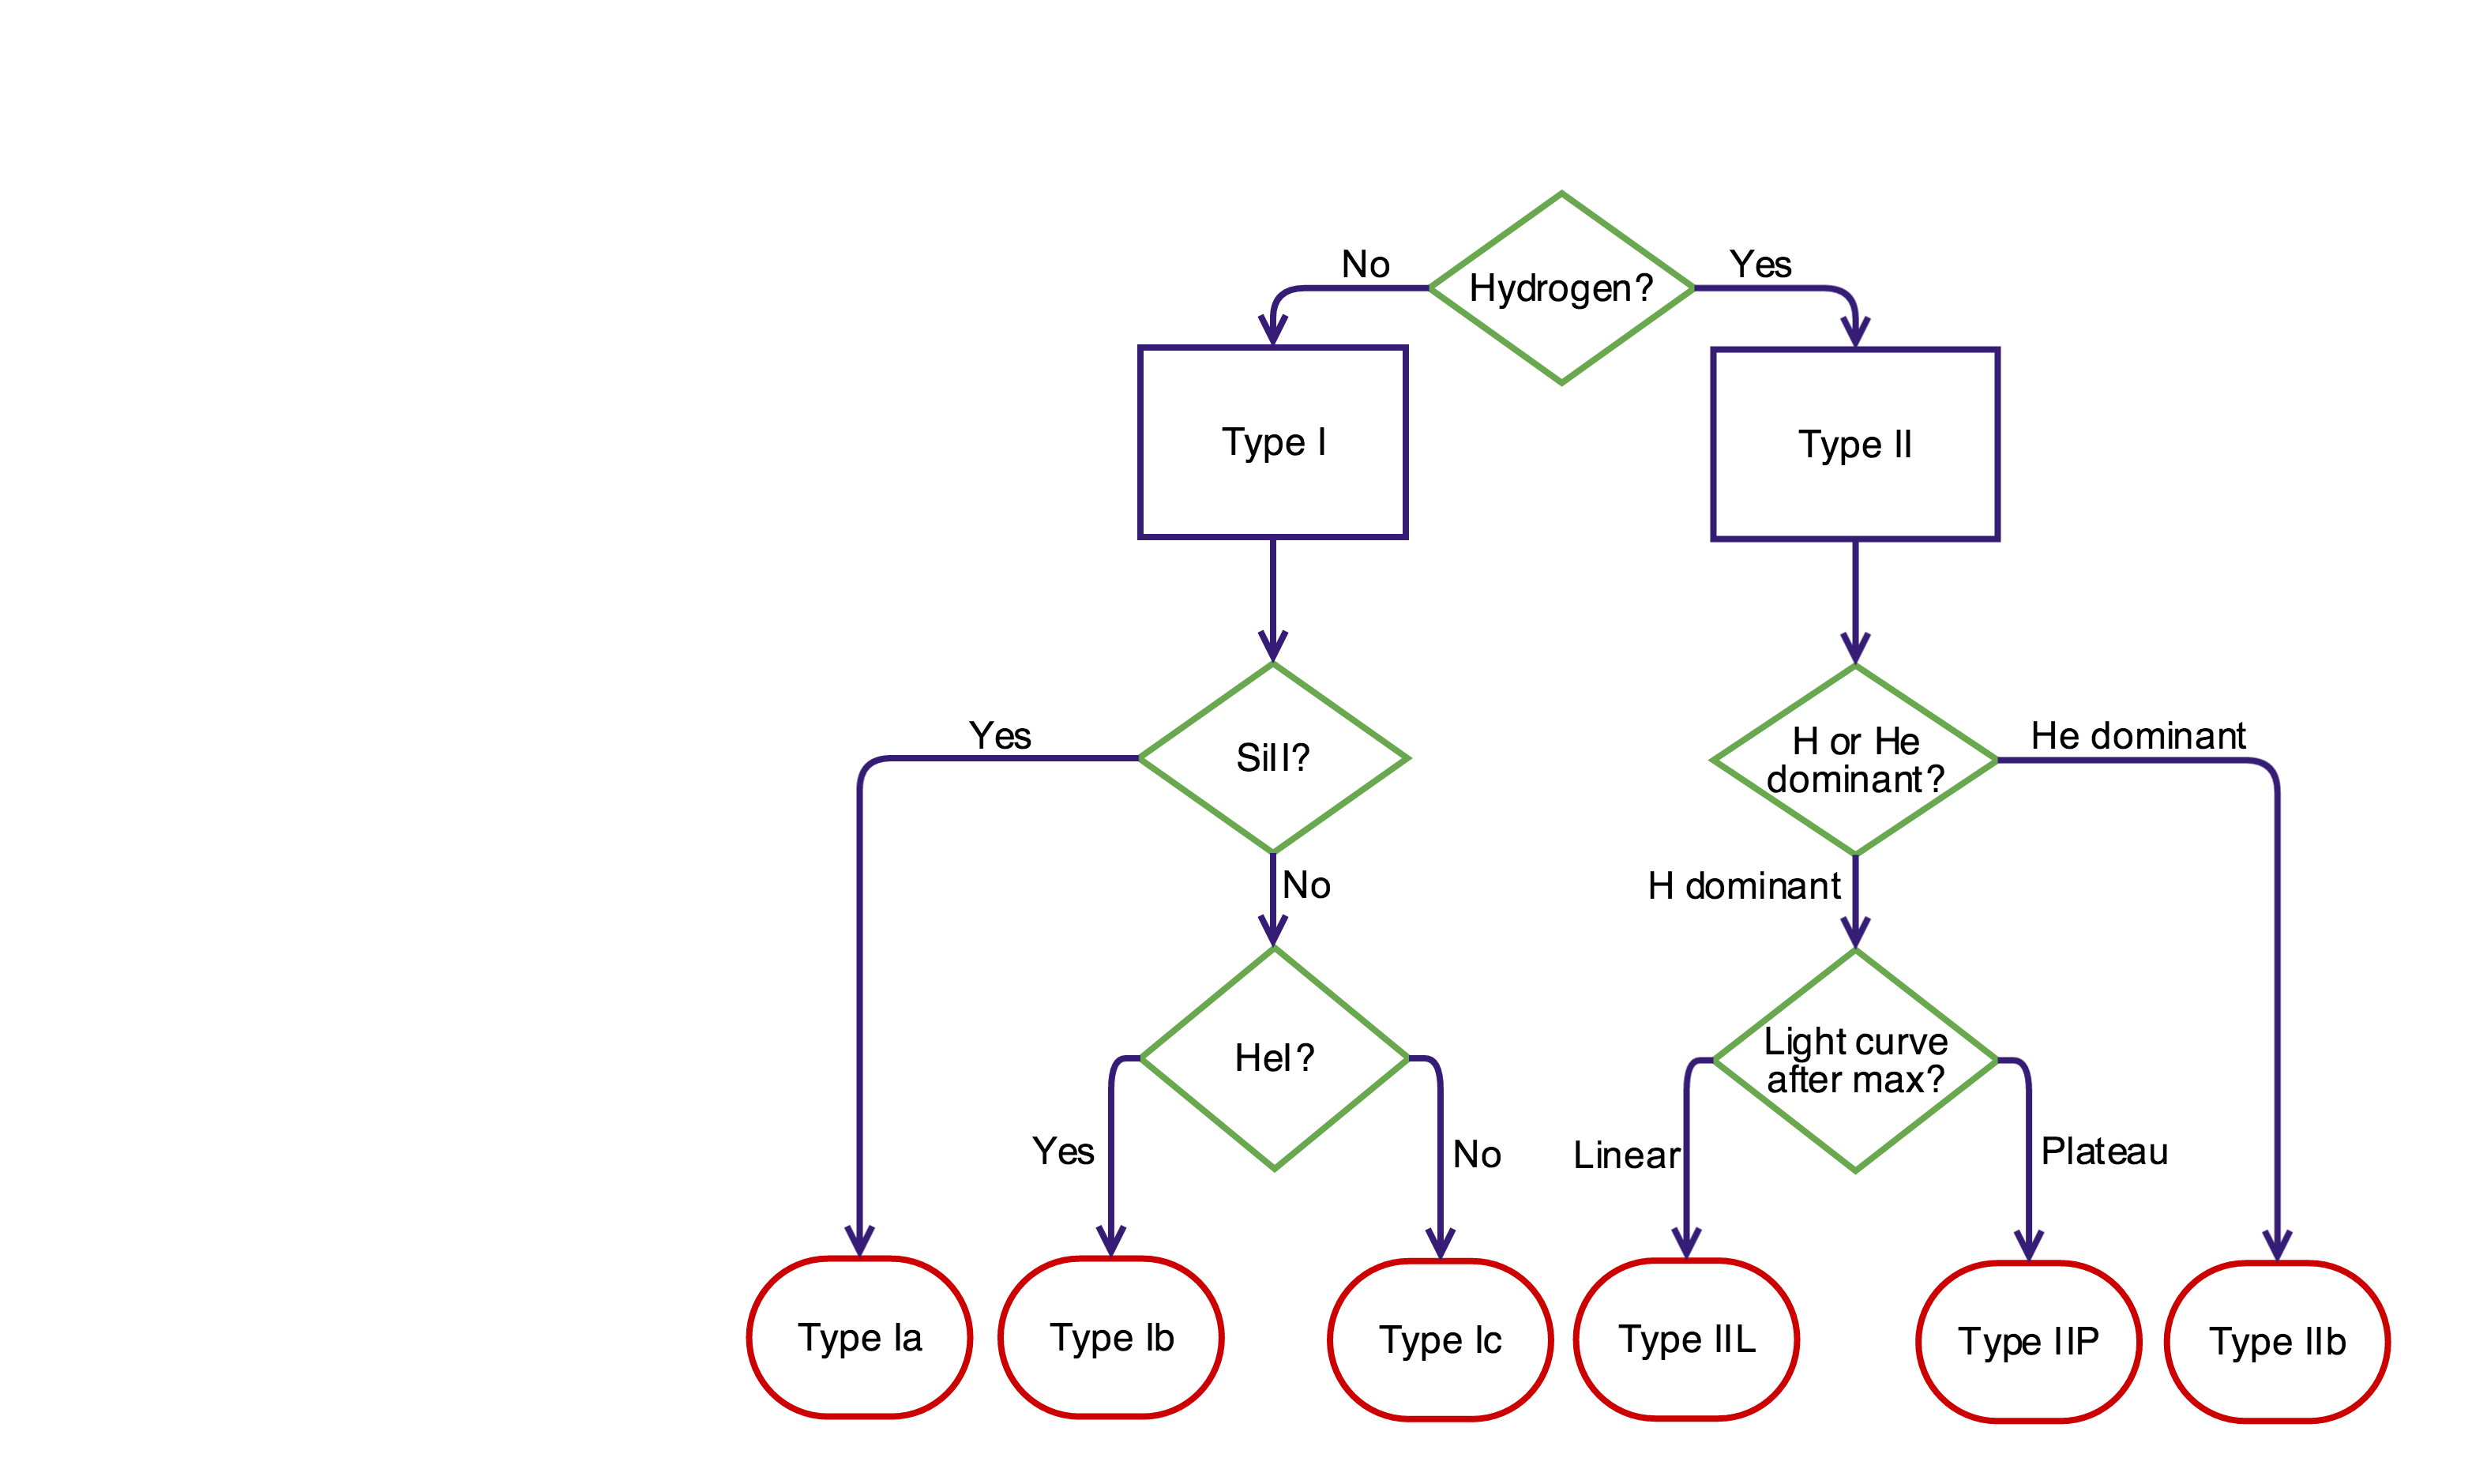
\includegraphics[clip=true, scale = 0.2, trim= 930 50 55 210]{chapters/chapter1/figs/sn_classification.png}
\caption{A flowchart summarising the supernova classification scheme}
\label{intro:fig:sn_class}
\end{figure}


%THIS IS MESSY
The initial classification of Type I or Type II is based on very early spectra, as are all further classifications of Type I supernovae.  Type II supernovae are more complex in their categorisation.  The further subdivisions of the Type II supernovae depend on the dominance of hydrogen or helium in later spectra, with helium dominant supernovae being classified as Type IIb.  The classification of Type II supernovae that exhibit strong hydrogen lines is then dependent on the evolution of the light curve after maximum light, with a linearly decaying light curve being classified as Type IIL and a plateauing light curve classifying the supernova as Type IIP.  Type IIn supernovae are omitted from the summary presented in Figure \ref{intro:fig:sn_class} as they cannot be classified straightforwardly via a bifurcating process.  Type IIn supernovae will generally have strong emission lines, particularly hydrogen lines, often with complex profiles.  Crucially, the spectra of Type IIn supernovae do not exhibit the broad absorption features frequently seen in other types and instead contain narrow lines (hence Type IIn).  

\subsection{From Massive Stars to Remnants}
%make this flow more nicely :)

It is generally accepted that the progenitors of Type Ia supernovae are white dwarfs that exist in a binary system with another star.  The accretion of material from one star to another results in a thermonuclear explosion.  This explosion mechanism is unique to Type Ia supernovae with Type Ib/c and Type II supernovae thought to explode via the core-collapse mechanism.  Broadly, this process is initiated when the massive star ($\ge 8$\msun) starts to fuse heavier elements. The fusion of ever heavier elements generates less and less energy whilst also causing the mass of the core to increase.  Eventually, radiation pressure drops sufficiently that the core can no longer support itself against its own self-gravity and begins to collapse rapidly. Within milliseconds, the core reaches extremely high densities and, when it can no longer condense further, ``bounces" off itself causing both an immense shockwave to propagate outwards and a vast quantity of energy to be released via the expulsion of neutrinos.  Much of this complex process is still poorly understood and interesting work is currently being done modelling these very early stages.  Though the explosion mechanisms of CCSNe are largely beyond the scope of my work, some attention will be paid to these models later in this thesis since instabilities that arise in these early stages can influence the structure of the ejecta at later stages of its evolution.

For several hundred years after the explosion, the supernova (now a remnant) is in the free-expansion phase. During this phase, the mass and velocity of the expanding supernova massively exceed those of the surrounding medium and the behaviour of the remnant may be analysed as if it were expanding into a vacuum.  The shock radius during this phase may be simply calculated as $R_s = v_s t$.  As the shockwave propagates through the ISM, interstellar material that has been compressed by the forward shock begins to accumulate.  At the same time a reverse shock wave begins to propagate back through the ejecta.  It is during this phase, which arises very soon after the initial explosion and lasts for a few hundred years, that the physical conditions in the ejecta are thought to be optimal for dust formation.


\subsection{Dust Formation in CCSNe}

Superficially, the formation of dust grains requires densities high enough for interaction between particles to take place, but temperatures that are cool enough to allow the grains to survive.  The theory that the ejecta of a CCSN in its free-expansion phase could provide these conditions  was first hypothesised by \citeauthor{Cernuschi1967} in 1967 and they have now long been thought to be potential dust factories \citep{Hoyle1970, Kozasa1991, Todini2001}.  

The formation of dust was originally thought to result from the stochastic process of classical nucleation whereby particles coalesce to form the seeds of dust grains.  These seeds become the nucleation sites from which grains are ultimately born through the aggregation of further particles.  Various models of dust formation in the ejecta of CCSNe have used this approach \citep{Kozasa1989, Todini2001,Nozawa2003, Schneider2004}.  

More recently, several models of dust formation in CCSNe that consider the effects of chemistry on the growth of dust grains have been published.   These models consider the chemical composition of the gas and include chemical reaction rates thereby considering the manner in which molecular evolution influences dust grain formation and growth rates \citep{Cherchneff2009, Cherchneff2010, Sarangi2013, Sarangi2015}.

Models using both methods have predicted dust masses of the order of 0.1-1\msun of dust forming within the ejecta of CCSNe of progenitor masses between 12-40\msun within the first few years after the initial explosion.

\subsection{The Three Signatures of Dust}

The presence of dust in the ejecta of CCSNe can be indicated by three main signatures: 

\subsubsection{A decrease in the light curve} 
As the dust begins to form in the ejecta, UV and optical light is absorbed by the dust causing a decrease in the light curve at these wavelengths.

\subsubsection{Excess IR emission}
An increase in emission in the IR occurs contemporaneously with the decrease in the UV-optical light curve.  A thermal MIR excess is caused by warm dust and an excess in the far-IR and sub-mm is the result of cold dust.  The increase in emission in these wavelength can be caused by newly-formed dust condensing in the ejecta but can also be a result of the illumination of pre-existing dust

\subsubsection{Blue-shifted line profiles}
Finally, the onset of the formation of dust can cause an asymmetry in line profiles in the optical and IR.  The absorption and scattering of optical or near-IR radiation by newly-formed dust within the ejecta can result in an asymmetry between the red and blue shifted components, with redwards 
emission from the far side of the ejecta undergoing greater absorption and resulting an overall shift of the profile to the blue.
\\

\noindent All three of these signatures have been discussed in detail over the timeline of this subject but the focus has been on using the excess IR emission seen in the SED of CCSNe to determine quantitatively dust masses in these objects.  This approach has resulted in a lively debate regarding the quantities of dust that CCSNe are capable of producing.
 
\subsection{The Dust Mass Debate}

%%MAYBE MORE DETAIL HERE %%%%
Over the past two decades, several high redshift galaxies  have been found to contain significant masses of dust \citep{Omont2001, Bertoldi2003, Watson2015}.  CCSNe are one of the few potential sources that could contribute large quantities of dust at early epochs. However, 
observations over the last decade at mid-infrared (MIR) wavelengths of 
warm dust emission from CCSNe has suggested that the quantities of ejecta-condensed dust 
produced during the first 1000 days were typically $\leq$ 10$^{-3}$~M$_\odot$  
\citep{Sugerman2006, Meikle2007, Kotak2009, Andrews2010, Fabbri2011}.  This is much less than the 0.1-1.0~M$_\odot$ of dust per CCSN  
estimated to be needed  in order to account for the masses observed \citep{Morgan2003, Dwek2007}.  These observations would indicate that other early-time sources of dust must be found.

 However, recent {\em Herschel} far-IR and sub-mm observations of  several young supernova remnants have revealed cold dust  masses as high as 
0.2-0.8$M_{\odot}$, resulting in a 
re-evaluation of the rate of dust production by CCSNe and a renewed focus on these objects as sources of dust \citep{Barlow2010, 
Matsuura2011, Gomez2012}.

\subsubsection{SN 1987A}


%more waffle on sn1987a

Critical to this field has been the study of SN 1987A.   This supernova is one of the most studied objects in the history of astronomy and has been observed almost continuously since it exploded 28 years ago.  The reason for this is its proximity.  At only Xpc away, it has allowed for some exceptionally well-resolved spectral and photometric observations.  Neutrinos from its explosion were even detected by scientists at Y.  As such, it has yielded results and insight that would not have been possible otherwise and is a key to understanding the formation and evolution of dust in CCSNe.

It is of no surprise therefore that this object has been central to the debate.  \citet{Lucy1989} was the first to suggest the presence of dust in SN~1987A {\em Herschel} observations of SN~1987A were the first to suggest the presence of cold dust in any supernova.



\subsection{Motivation - call something else}

It is seems increasingly likely that CCSNe do indeed produce significant quantities of dust.  However, there remain a large number of outstanding challenges to consider.  Firstly, there are still only a very small number of supernovae that have been observed to have sizeable masses of dust present in their ejecta.  If further CCSNe were also shown to have formed large quantities of dust then  the already shifting opinion might start to become consensus.  Other points to consider regarding dust formation and evolution in CCSNe include the nature of the dust (composition, grain size, grain shape etc.) which is still largely unclear, as is the extent to which it is destroyed or sputtered after its initial formation.  Related to this is the uncertainty of the dust formation rate in the ejecta and the issue of where this formation takes place.  These are all interesting questions that call out for answers.  

The {\em Hershel} dust mass estimates were based on fitting dust SEDs that peaked at far-IR wavelengths. Unfortunately, following the end of the {\em Herschel} mission in 2013, there is likely to be a long wait for far-IR facilities with comparable or better sensitivities than {\em Herschel} to become available.  Without data, this methodology is temporarily ineffectual.  This provided an incentive to make use of alternative methods to estimate the dust masses that form in supernova ejecta.

\section{Dust-Affected Line Profiles}

%%MORE HERE

The purpose of my work has been to develop a new approach to determining dust masses in supernovae, with the aim of providing an alternative to SED fitting for the future and of providing corroborating or contradicting evidence of past results.  I looked to exploit the third signature of dust formation in supernovae, namely the red-clue line asymmetry observed in optical and IR line profiles.  Though this feature has been discussed a length by numerous authors (REFERENCES) it has very rarely been quantitatively measured or modelled.

I have sought to construct a Monte Carlo based code that numerically models this feature in the spectra of SNe in order to quantitatively determine dust masses formed at a variety of epochs post-explosion, additionally seeking to place constraints of the composition and grain size distributions of the newly-formed dust.

\subsection{Observing}

Numerous telescopes have recorded spectra of CCSNe in the optical and IR, some with extremely high resolution.  The Anglo-Australian Telescope (AAT), the Cerro Tololo Inter-American Observatory (CTIO), the Hubble Space Telescope (HST) and the Very Large Telescope (VLT) have all observed several supernovae in the optical including SN 1987A.  Other telescopes such as  the two Gemini Multi-Object Spectrographs (GMOS) have also taken spectra of numerous CCSNe.

Advances in digital storage have allowed for spectral and photometric observations to be made easily available online.  Many observatories now publish their recent observations online in archives and are working to upload observations that pre-date file sharing services.  Much of the data used in this thesis was obtained from these archives. 

\subsection{Previous Work on Line Profiles}
LUCY LUCY LUCY!!!  Also some of the other stuff - gerasimovic, some of the other theoretical papers, maybe also the electron scattering stuff


EXAMPLES OF RBLA WORK
\subsection{Modelling}
Need to think about what i actually need to consider in this section.

- dust absorption, scattering and reemission in the IR
- raditaive transfer and independence of optical properties and temp meaning do not need to fully solve rad tran problem
- mie theory deets?  how is it solved and what is the theory?
- assumptions of isotropy?  scattering matrices?
\subsection{Mie Theory}

In order to truly understand observations that are a product of dust, we must first understand those facets of a dusty medium that determine its interaction with incident radiation.  Dust grain radii are often of a similar order of magnitude to the wavelength of that incident radiation and so may be analysed from an optical perspective using Mie Theory.  Mie Theory is a mathematical solution to Maxwell's equation that describe how light is scattered off a small particle.  In combination with the optical properties of the medium, this allows for a precise determination of the extinction and scattering efficiencies of a given environment.  Conveniently, this allows for the straightforward modelling of a dusty medium and it is this calculation that I exploit in my models.  Mie Theory assumes particles to be spherical, an assumption which is a potential issue since grains may be crystalline, fluffy or extremely amorphous.  This issue is addressed later in this thesis.



\section{This Thesis}
And relate to your current work - give an overview of the work and what you did as well as the structure of the thesis - see Jo's for example.
